\documentclass[12pt]{article}
\bibliographystyle{plain}
\usepackage[utf8]{inputenc}
\usepackage{graphicx}
\usepackage{subfigure}
\title
{MSMBuilder 2.5 Tutorial
}
\begin{document}

\maketitle

\section{Table of Contents}
\begin{enumerate}
\item Installation
\item Using MSMBuilder
\item MSMBuilder Tutorial
\item Frequently Asked Questions
\end{enumerate}

\newpage

\section{Installation}

\subsection{Prerequisites}
\begin{itemize}
 \item CPU with SSE3 support.
\item GCC 4.2 or later (with OpenMP support)
\item Python
\item Numpy
\item Scipy
\item PyTables
\item numexpr
\item fastcluster
\item matplotlib (optional for plotting)
\item ipython (optional for interactive mode)
\item pymol (optional for visualization)
\end{itemize}
Note that the Enthought Python Distribution contains most of these prerequisites and provides an easy way to facilitate installation.

\subsection{Install Python and Python Packages}

Rather than individually install the many python dependencies, we recommend that you download the Python2.7 version of the Enthought Python Distribution, which contains all python dependencies required to run MSMBuilder.  Please use the 64 bit versions, as this will give higher performance in our RMSD code.

Note for OSX users: Enthought represents the easiest way to obtain a working Python installation.  The OSX system Python install is broken and cannot properly build Python extensions, which are required for MSMBuilder installation.

Note: please use a 64 bit version of python (and thus of MSMBuilder).  On certain systems (OSX Lion), 32 bit builds have experienced crashes in the RMSD / Clustering code.

\subsection{Download and Install MSMBuilder}

Download MSMBuilder, unzip, move to the msmbuilder directory.  Install using setup.py:
\begin{verbatim}
python setup.py build
python setup.py install
\end{verbatim}

You may need root privileges during the install step; alternatively, you can specify an alternative install path via --prefix=XXX.  If you performed the install step with “--prefix=XXX”, you need to ensure that

1.  XXX/bin is included in your PATH
2.  XXX/lib/python2.7/site-packages/ is included in your PYTHONPATH

Step (1) ensures that your can run MSMBuilder scripts without specifying their location.  Step (2) ensures that your Python can locate the MSMBuilder libraries.  

\newpage

\section{Using MSMBuilder}

MSMBuilder has been designed to provide both ease of use and versatility.  To achieve both these goals, we have pursued a 2-pronged approach.

\begin{enumerate}
\item MSMBuilder is a library.
\item MSMBuilder is a set of python scripts.  
\end{enumerate}

Using MSMBuilder as a library allows for fast but powerful customization.  Using MSMBuilder as a library is recommended only for advanced users and is described in the MSMBuilder Scripting Guide.

MSMBuilder contains a suite of python scripts that automate the most common tasks in model construction.  For most situations, conformational dynamics can be modeled with the following protocol.  Each script below provides instructions by running with the -h flag.  Note that setup.py should have installed each script below to someplace in your PATH.  

\subsection{MSMBuilder Scripts}
\subsubsection{ConvertDataToHDF.py}

Merges XTC files into continuous HDF5 files that MSMB2 can read quickly.  Takes data from a directory of trajectory directories or a FAH-style filesystem.  

Note: if you wish to convert a pre-existing MSMBuilder1 project, use UpdateProjectToHDF5.py 

\subsubsection{CreateAtomIndices.py}
Selects atom indices you care about and dumps them into a flat txt file. Can select all non-symmetric atoms, all heavy atoms, all alpha carbons, or all atoms.

\subsubsection{Cluster.py}
Clusters your data based on RMSD using a novel hybrid k-centers / k-medoids algorithm. It is recommend that you subsample data at a timestep similar to (~10X) the desired lagtime of your eventual model (over-subsampling can lead to kinetic barriers within states). Choose a clustering diameter (-D) suitable for your system.  We find that for folding simulations of villin, a diameter of 0.175 nm led to a high resolution model.  We recommend approximately 10 iterations of the (local) hybrid k-medoid clustering.  Additional iterations of local and global hybrid clustering may lead to slightly reduced discretization error (up to 25% improvement), but at the cost of significantly longer clustering times.  
	NOTES:
-The hybrid k-medoids clustering works by simultaneously minimizing both the average-case and worst-case clustering errors.  Email kyle for details / MSMBuilder2 draft.
- Stride is in units of frames to subsample. It will subsample whatever is in your Trajectories/ directory, so if you subsampled in the ConvertToHDF.py script then this will subsample the subsample.

\subsubsection{Assign.py}
Assigns data to the cluster generators. Use AssignOnPBS.py and MergeAssignOnPBS.py to parallelize this process on a PBS-based cluster (highly recommended!).

\subsubsection{CalculateImpliedTimescales.py}
Calculates the implied timescales for a python range of MSM lag times. This is equivalent to the old BuildMSMsAsVaryLagTime.py. Can be used on Micro or Macro scale models.  
	NOTES:
  	- You might get a SparseEfficiencyWarning for every lag time. Ignore this.
	- Lagtimes are input as frames that have been assigned, i.e. Those you have converted to HDF5
	
\subsubsection{PlotImpliedTimescales.py}
A template for generating an implied timescales plot.

\subsubsection{BuildMSM.py}
Estimate a reversible transition and count matrix using a three step process:

1. Merge states with low counts to improve statistics
2. Use Tarjan algorithm to find the maximal strongly-connected (ergodic) subgraph
3. Use MLE (e.g. Boxer iteration) to estimate a reversible count matrix consistent with your data.

This script also outputs the equilibrium populations of the resulting model.

\subsubsection{GetRandomConfs.py}
Rips random conformations from each state of your MSM. This is very useful for efficient calculation of observables.

\subsubsection{CalculateClusterRadii.py}
Calculates the mean RMSD of all assigned snapshots to their cluster generator for each cluster. Gives an indication of how structurally diverse clusters are.

\subsubsection{CalculateRMSD.py}
Uses MSMb2's rapid RMSD calculator to calculate the RMSD of your trajectories/generators/assignments. Very useful for deciding which clusters belong to the folded, unfolded, or transition state ensembles (or any other grouping!)

\subsubsection{CalculateProjectRMSD.py}
Calculates the RMSD of all conformations in a project to a given conformation.

\subsubsection{DoTPT.py}
Performs Transition Path Theory (TPT) calculations. You will need to define good starting (reactants/U) and ending (products/F) ensembles for this script. Writes the forward and backward committors and the net flux matrix

\subsubsection{SavePDBs.py}
Allows you to rip random PDBs from your project and save them to disk.

\subsubsection{PCCA.py}
Perron Cluster-Cluster Analysis (PCCA) clusters Microstates into Macrostates. This script generates a new, macro-level assignments file from a microstate model. (Use Assignments.Fixed.h5) The simplex version can be specified. This version is more robust, but more resource-intensive. See the main discussion of macrostate models in XXX.

\newpage

\section{Tutorial}
\subsection{MSM Construction}

\subsubsection{Overview of MSM Construction}
Constructing a Markov State model involves several steps, which are summarized below:
\begin{enumerate}
 \item Simulate the system of interest.
 \item Convert trajectory data to MSMBuilder format.
 \item Cluster and assign your data to determine microstates.
 \item Construct a microstate MSM
 \item Calculate macrostates using (f)PCCA+
 \item Calculate a macrostate rate matrix using SCRE
 \item Validate the resulting model.
\end{enumerate}

\subsection{Alanine Dipeptide Tutorial}

This section walks users through a complete Markov state model analysis of the Alanine Dipeptide data provided in MSMBuilder.

In the following, we assume that you have properly installed MSMBuilder.  We also assume that you unzipped the MSMBuilder source file into directory ~/msmbuilder/.  If you unzipped the file elsewhere, you will need to change the paths accordingly.  

Finally, in this tutorial we assume that you have installed pymol for viewing conformations.

\subsubsection{Move to tutorial directory, prepare trajectories}
\begin{verbatim}
cd $PREFIX/share/msmbuilder_tutorial 
tar -xvf XTC.tar
\end{verbatim}

Here, $PREFIX$ is the base directory of your msmbuilder installation.

\subsubsection{Create an MSMBuilder Project}
\begin{verbatim}
ConvertDataToHDF.py  -s native.pdb -i XTC
\end{verbatim}

\subsubsection{Cluster your data}
WARNING: this step requires a minimum of 3.0 GB of memory for storing a matrix of pairwise RMSD.
\begin{verbatim}
Cluster.py rmsd hierarchical -h -m ward
\end{verbatim}

\subsubsection{Assign data to states}

\begin{verbatim}
AssignHierarchical.py -H Data/Zmatrix.h5 -n 100
\end{verbatim}

\subsubsection{Validate model with relaxation timescales.}
We calculate the relaxation timescales for a sequence of lagtimes $\{1, 2, ..., 50\}$:
\begin{verbatim}
CalculateImpliedTimescales.py -l 1,25 -i 1 -o Data/ImpliedTimescales.dat
\end{verbatim}

Next, we use python to plot the results, specifying the lagtime between frames (1 ps):  

\begin{verbatim}
PlotImpliedTimescales.py -d 1. -i Data/ImpliedTimescales.dat
\end{verbatim}

\subsubsection{Construct MSM at appropriate lagtime}
The plotted relaxation timescales suggest that the three slow timescales are reasonable flat at a lagtime of 3 timesteps [ps].  Thus, we construct an MSM using that lagtime:

\begin{verbatim}
BuildMSM.py -l 3 
\end{verbatim}

At this point, MSMBuilder has written the following files into your ./Data/ directory:

Assignments.Fixed.h5
tCounts.UnSym.mtx
tCounts.mtx
tProb.mtx
Mapping.dat
Populations.dat

Assignments.Fixed.h5 contains a “fixed” version of your microstate assignments that has removed all data that is trimmed the maximal ergodic subgraph of your data.  

tCounts.UnSym.mtx contains the raw counts of the ergodic data.  These counts may not be reversible (thus, the count matrix may not be symmetric).  

tCounts.mtx contains the maximum likelihood estimated reversible count matrix.  This is a symmetric matrix.  

tProb.mtx contains the maximum likelihood estimated transition probability matrix.  

Mapping.dat contains a mapping of the original microstate numbering to the “fixed” microstate numbering.  This is necessary because some states may have been discarded during the ergodic trimming step.  

Populations.dat contains the maximum likelihood estimated reversible equilibrium populations.  

\subsubsection{Construct a Macrostate MSM}

Spectral cluster methods such as PCCA+ can be used to construct metastable models with a minimal number of states.  First, we need to construct a microstate model with a short lagtime.  The short lagtime is necessary because PCCA+ tries to create macrostates that are long-lived, or metastable.  At long lagtimes, states become less and less metastable.  

\begin{verbatim}
 BuildMSM.py -l 1 -o Lagtime1
\end{verbatim}

Our previous examination of the relaxation timescales suggested that there were 3 slow processes, so we choose to build a model with 4 macroscopic states.  

\begin{verbatim}
PCCA.py -n 4 -a Lagtime1/Assignments.Fixed.h5 -t Lagtime1/tProb.mtx -o Macro4/ -A PCCA+
\end{verbatim}

\subsubsection{Examining the macrostate decomposition}

It is known that the relevant degrees of freedom for alanine dipeptide are the phi and psi backbone angles.  Thus, it is useful to examine (phi,psi), which we have pre-calculated for you.

\begin{verbatim}
./PlotDihedrals.py Macro4/MacroAssignments.h5
\end{verbatim}

You should see the following graph:
\begin{center}
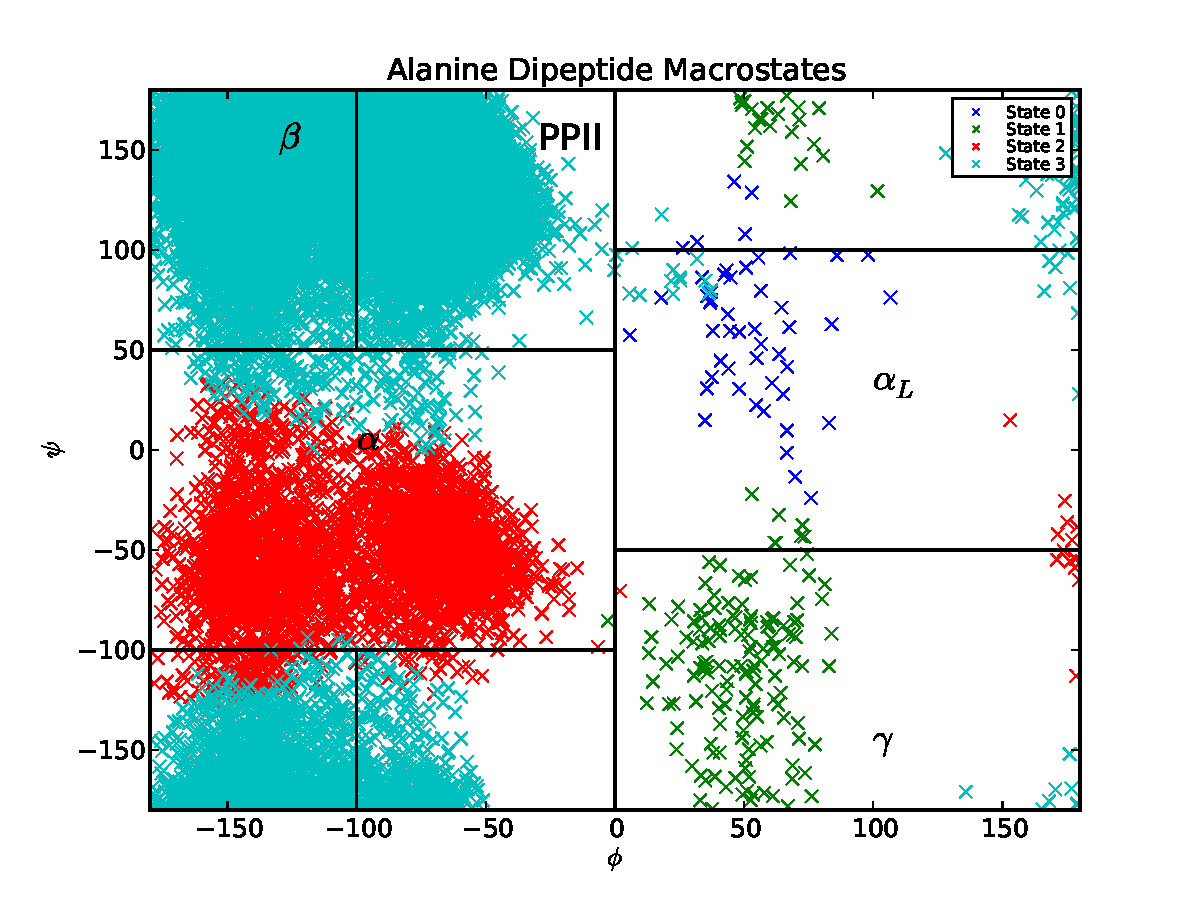
\includegraphics[width=6.7cm]{figures/Macro4}
\end{center}


Thus, the PCCA algorithm has automatically identified the key basins of alanine dipeptide.  The black lines correspond to the $\beta, PP_{II}, \alpha_R, \alpha_L$ and $\gamma$ conformational basins, as estimated previously (Sosnick, 2005).  If we want a model that is less coarse grained, we can build a macrostate MSM with more states.  If, for example, we had used 5 states, we would produce a Ramachandran plot that also captures the barrier between the $\beta$ and $PP_{II}$ basins.  

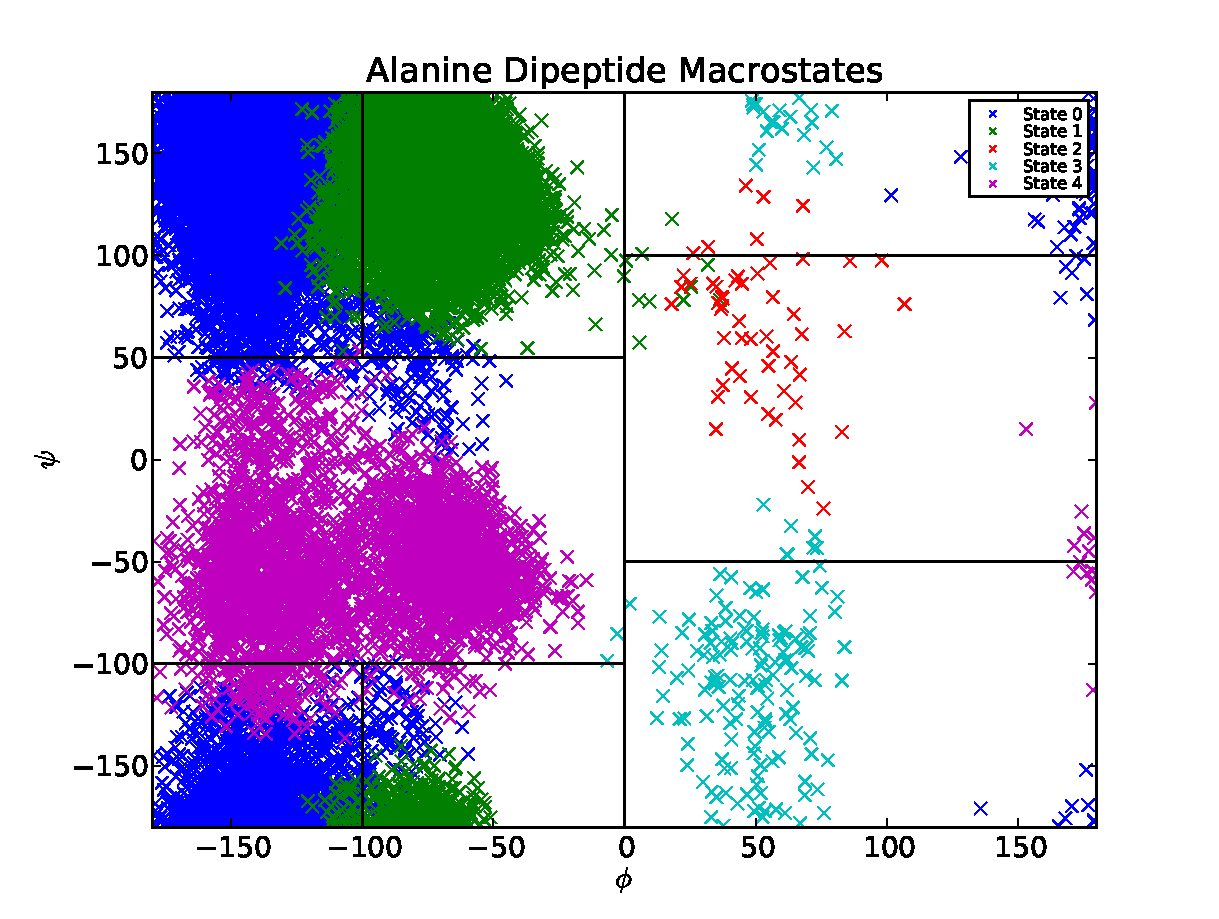
\includegraphics[width=6.7cm]{figures/Macro5}

In general, PCCA and PCCA+ are best applied to capturing long-lived, metastable states.  Thus, for this system, applying PCCA+ to construct models with more than 5 states may not produce useful models.  This is because alanine dipeptide only contains four eigenvalues that are significantly slower than the data resolution of 1 ps.  

\subsubsection{Calculate Macrostate Implied Timescales}

\begin{verbatim}
CalculateImpliedTimescales.py -l 1,25 -i 1 -o Macro4/ImpliedTimescales.dat -a Macro4/MacroAssignments.h5 -e 3
PlotImpliedTimescales.py -i Macro4/ImpliedTimescales.dat -d 1
\end{verbatim}

When using PCCA+, always verify two things:

\begin{enumerate}
 \item The state decomposition makes physical sense
 \item The macrostate implied timescales ``follow'' the microstate implied timescales
\end{enumerate}

The second point is important to check because occasionally, PCCA+ will lead to a degenerate solution.

\subsubsection{Estimate a converged rate matrix using SCRE}

In the macrostate implied timescales, the slowest implied timescale converges at approximately 10 ps, while the third timescale converges as 5 ps.  Furthermore, the third timescale is aliased at lagtimes starting with 13 ps; lagtimes longer than 13 ps will not accurately capture the dynamics of this relaxation.  This suggests that this system might benefit from estimating rates using SCRE and multiple lagtimes.  

To build an SCRE model, we first construct a macrostate transition matrix with lagtime 1.  

\begin{verbatim}
 BuildMSM.py -l 1 -a Macro4/MacroAssignments.h5 -o Macro4/
\end{verbatim}

Next, run the script GetRates-SCRE.py.  This script can be modified for use on arbitrary systems.  The key idea in SCRE is to estimate rate matrix $K_{ij}(\tau)$ for a variety of lagtimes.  Then, each rate matrix element is fixed when $K_{ij}(\tau)$ becomes approximately constant with respect to the lagtime $\tau$.  The final rate matrix provides estimates of Markovian rates for each of the rate elements $K_{ij}$.  Finally, PlotMacroStateImpliedTimescales.py can be used to compare the fixed-lagtime and SCRE estimates of implied timescales.  In practice, we find that the SCRE estimates capture the ``converged'' values of the fixed-lagtime timescales.  

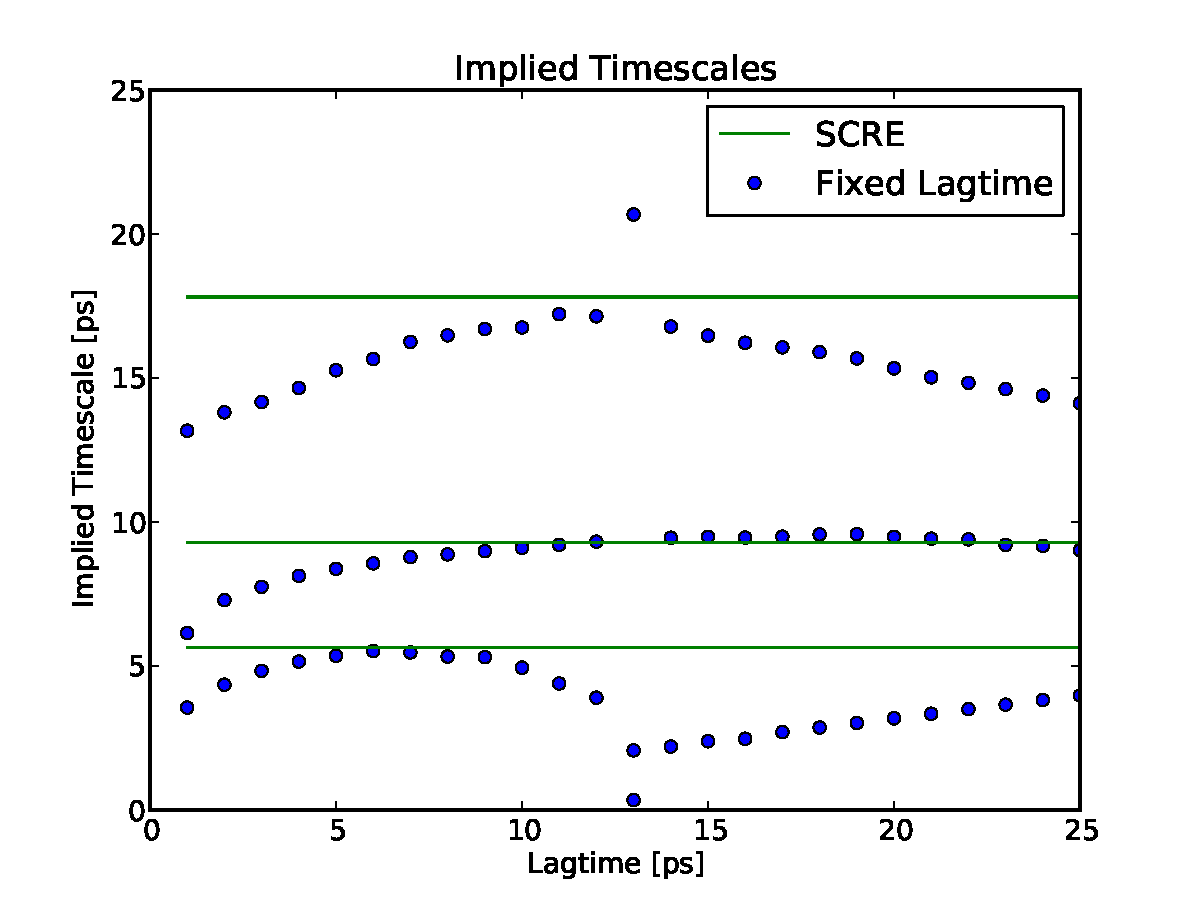
\includegraphics[width=6.7cm]{figures/SCRE}

\newpage

\section{Frequently Asked Questions}

Q1.  How do I decrease / increase the number of threads used during clustering, assignment, and rmsd calculation?

A1.  Set the \begin{verbatim}OMP_NUM_THREADS\end{verbatim} environment variable to the desired number of threads.  In linux, you would type (or add to your bashrc):
\begin{verbatim}
export OMP_NUM_THREADS=6 
\end{verbatim}

\vspace{5mm}

Q2:  I see the following error.  What do I do?
\begin{verbatim}
 #004: H5Z.c line 1095 in H5Z_pipeline(): required filter is not registered
\end{verbatim}

A2:  You are trying to read an HDF5 file that was written using a different PyTables installation.  Your current PyTables installation is likely missing the compression algorithm (filter) required to read the file.  The solution is to find a version of Pytables that has the old compression algorithm (filter) and use MSMBuilder to read and then re-write the trajectories (by default, MSMBuilder uses the PyTables BLOSC compression).  To do this (for a single File), you would so something like:
from msmbuilder import Trajectory
R1=Trajectory.Trajectory.LoadFromLHDF(Filename)
R1.SaveToLHDF(NewFilename)

\vspace{5mm}

Q3: I received an “Illegal instruction” error.  What does this mean?

A3:  MSMBuilder2 requires an SSE3 compatible processor when Clustering and calculating RMSDs.  Any processor built after ~2006 should have the necessary instructions.  

\vspace{5mm}

Q4:  In my implied timescales plot, I see unphysically slow timescales.  

A4:  The current estimators for transition matrices are somewhat sensitive to poor statistics.  The hybrid k-centers / k-kmedoids clustering focuses on providing the best possible clustering--without regard to the quality of the resulting statistics.  Thus, to get more precise timescales, you may have to find a way to achieve better statistics.  Here are a few ideas:
	A.  Collect longer trajectories.
	B.  Use fewer states.  Also, by increasing the number of local and global k-medoid updates, you can often increase the accuracy of your clustering while simultaneously lowering the number of states.  
	C.  Subsample your data when clustering.
	D.  Skip the initial k-centers step of clustering, instead using randomly selected conformations.  This generally leads to poorer clustering quality, but considerably better statistics in each state.  (Thus, the clusters will be much more localized to regions of high population density.)  This can be achieved by setting “-r 0” when clustering.  

\vspace{5mm}

Q5.  Why are there -1s in my Assignments matrix?

A5.  We use -1 as a “padding” element in Assignment matrices. Suppose your project has maximum trajectory length of 100.  If trajectory 0 has length 50, then A[0,50:] should be a vector of -1.  Furthermore, when you perform trimming to ensure (strong) ergodicity, futher -1s could be introduced at the start or finish of the trajectory.  Finally, if Ergodic trimming was performed with count matrices estimated using a sliding window, you could even see something like:
-1 -1 -1 x -1 -1 y z …
This is because sliding window essentially splits your trajectory into independent subtrajectories--one for each possible window starting position.  “x” then marks the start of one of these subtrajectories.


\end{document}